\documentclass[twoside,11pt,openright]{report}

\usepackage[utf8]{inputenc}
\usepackage[american]{babel}
\usepackage{a4}
\usepackage{latexsym}
\usepackage{amssymb}
\usepackage{amsmath}
\usepackage{amsthm}
\usepackage{epsfig}
\usepackage[T1]{fontenc}
\usepackage{lmodern}
\usepackage[labeled]{multibib}
\usepackage{color}
\usepackage{datetime}
\usepackage{epstopdf} 
\usepackage{cleveref}
\usepackage{geometry}
\usepackage{tikz}

\renewcommand*\ttdefault{txtt}

\newcommand{\todo}[1]{{\color[rgb]{.5,0,0}\textbf{$\blacktriangleright$#1$\blacktriangleleft$}}}
\newcommand{\DIST}{\operatorname{DIST}}

\newcommand{\substr}[3]{#1\langle #2, #3 \rangle}
\newcommand{\str}[3]{#1[#2, #3]}
\newcommand*{\circled}[1]{\tikz[baseline=(char.base)]{
                          \node[shape=circle,draw,inner sep=2pt] (char) {#1};}}

\newcites{A,B}{Primary Bibliography,Secondary Bibliography}

\newtheorem{mydef}{Definition}
\newtheorem{lemma}{Lemma}
\newtheorem{claim}{Claim}

% see http://imf.au.dk/system/latex/bog/

\begin{document}

%%%%%%%%%%%%%%%%%%%%%%%%%%%%%%%%%%%%%%%%%%%%%%%%%%%%%%%%%%%%%%%%%%%%%%%

\pagestyle{empty} 
\pagenumbering{roman} 
\vspace*{\fill}\noindent{\rule{\linewidth}{1mm}\\[4ex]
{\Huge\sf Computation of Edit Distance in Compressed Strings}\\[2ex]
{\huge\sf Kasper Nielsen, 20091182}\\[2ex]
\noindent\rule{\linewidth}{1mm}\\[4ex]
\noindent{\Large\sf Master's Thesis, Computer Science\\[1ex] 
\monthname\ \the\year  \\[1ex] Advisor: Christian Nørgaard Storm Pedersen\\[15ex]}\\[\fill]}

\epsfig{file=logo.eps}\clearpage

%%%%%%%%%%%%%%%%%%%%%%%%%%%%%%%%%%%%%%%%%%%%%%%%%%%%%%%%%%%%%%%%%%%%%%%

\pagestyle{plain}
% \chapter*{Abstract}
% \addcontentsline{toc}{chapter}{Abstract}

% \todo{in English\dots}

% \chapter*{Resum\'e}
% \addcontentsline{toc}{chapter}{Resum\'e}

% \todo{in Danish\dots}

% \chapter*{Acknowledgements}
% \addcontentsline{toc}{chapter}{Acknowledgments}

% \todo{\dots}

% \vspace{2ex}
% \begin{flushright}
%   \emph{Kasper Nielsen,}\\
%   \emph{Aarhus, \today.}
% \end{flushright}

\tableofcontents
\pagenumbering{arabic}
\setcounter{secnumdepth}{2}

%%%%%%%%%%%%%%%%%%%%%%%%%%%%%%%%%%%%%%%%%%%%%%%%%%%%%%%%%%%%%%%%%%%%%%%

%\chapter{Introduction}
%\label{ch:intro}
%\todo{\dots}

\section{Introduction}
Focus on computation of edit distance. That is, insert / delete of cost 1, match of cost 0. This can be generalized to different classes of scoring functions, which in some cases results in more complicated algorithms with worse asymptotic running time and space consumption, even if the cost function is assumed to be computable in constant time.

Focus on how well strings can be compressed as SLPs, compared to other encodings ex BWT and entropy based compression algorithms (ex Huffman encoding). Try to think about algorithms that works for these other (presumably better) compression algorithms.

\section{Compression of strings}
Describe and discuss different types of string compression.
\begin{itemize}
  \item Information theoretical bound for compression, and encoding schemes satisfying this bound (ex Huffman encoding / Arithmetic coding).
  \item Definition of SLPs, and compression schemes transformable to SLPs (Z77, Z78, LZW).
  \item Other transformations possibly making subsequent compression more efficient (ex BWT)
  \item Compare how well the strings are compressed compared to the information theoretic lower bound given by the entropy.
\end{itemize}

\section{Simpel}
\todo{Give credit to some guy!}
A standard dynamic programming algorithm for solving the Edit Distance problem, is denoted the simple algorithm or simple implementation. It is given two string $A[1..n]$ and $B[1..m]$ for which the edit distance should be computed, and fills out a matrix of size $n \times m$ where a given entry $(i, j)$ corresponds to the edit distance between $A[1..i]$ and $B[1..j]$. The rules for filling out a table entry follows directly from the definition of edit distance when extending a string, and are as follows:
\todo{match, insert, delete}
The base case where a string is aligned to the empty string is trivially $0$. Therefore the edit distance between two string can be computed using both $O(nm)$ time and space. Notice that an easy optimization where only the last row used is stored in memory reduces the space consumption to $O(\min\{n, m\})$.

\subsection{Backtracking}
If the actual alignment(s) of the strings is desirable, it can be found by a standard back-tracking approach on the computed matrix.

This however implies that the simple space optimization from before does not work, as all entries in the computed table potentially is needed for the backtracking. However, a divide-and-conquer algorithm was given by Hirshberg\todo{Cite} that reduces the space consumption of $O(\min\{n, m\})$ without asymptotically increasing the running time.\todo{Describe the approach?}

\subsection{Optimizations}
Ideas:
\begin{itemize}
  \item Compute matrix only around its diagonal, and then extend if needed.
  \item Using SIMD instructions.
  \item Parallelization (CPU / GPU).
\end{itemize}

\section{Compression based algorithms}
A recent approach for speeding up the computation of edit distance, is to do some compression of the strings before aligning them, and then in some way do the edit distance computation using the compressed strings, which in many cases will be shorter than the original input.

\subsection{The 4 Russian Trick}
This approach was not originally presented as a compression based algorithm, but using that each entry in the dynamic programming matrix is changing at most 1 from an adjacent entry, and that the alphabet is finite, it is possible to encode blocks of the matrix space efficiently and pre-compute all of them. That is, for all different sub-strings and possible inputs to compute the relative outputs when applying the block. This is then used to fill out the original dynamic programming matrix block-by-block.
\todo{Describe details and analyze time complexity?.}

\subsection{Run-Length Encoding}
\begin{itemize}
  \item \todo{Describe RLE}
  \item Not the focus / implemented in this thesis, but the result is included for completeness. Refer old thesis for experimental results of this approach?
  \item \todo{cite} gave an algorithm running in time $O(nm)$ where $n$ and $m$ denotes the size of the compressed sequences. This is the first result where the running time is only depending on the length of the compressed strings. However, for string not containing long runs of the same symbol, RLE will generate strings longer than the original input!
\end{itemize}

\subsection{Compression based on SLPs}
This is the main focus of this thesis.

\newcommand{\SLP}[1] {\mathcal{#1}}

The algorithm is a bit like the 4 Russion Algorithm, however the blocking of the dynamic programming table is based on the productions of the SLPs, so that reused productions results in reusable blocks. The algorithm can be summarized in the following steps:
\begin{itemize}
  \item Construct a SLP representation $\SLP{A}$, $\SLP{B}$ of the two input strings $A$ and $B$. The better the compression scheme is able to compress the SLP representations the faster the algorithm will be. The running time of this scheme depends on the compression scheme employed, but using Z77, Z78 or LZW this can be in time $O(N)$ \todo{be sure, and cite?}.
  \item Select productions from the SLPs generating strings of length $O(x)$ for some fixed $x$ are selected in such a way that they cover the entire string without duplication. This can trivially be done in time $O(N)$ where also a list of selected productions is generated in such a way that the associated strings is the original input string.
  \item Blocks from the dynamic programming table (called DIST tables) are precomputed for all the selected productions. These DIST tables naively takes up can be represented using $O(x^2)$ space to represent, but using a succinct representation given in \todo{cite}, it is possibly to reduce the space consumption to $O(x)$ trading for a query-time of $\log^2 x$ time. This increased query time is also the reason the algorithm gains an extra $\log{x}$ factor, which is conjectured to be unnecessary \todo{cite}. Using the succinct representation and a the way of merging succinct DISTs from \todo{cite}, this step can be computed in time $O(n^2x\log{x})$.
  \item The dynamical programming table is filled up by using the generated partition of the string and then applying the DIST tables. This step takes time $O(\left(\frac{N}{x}\right)^2 \cdot AP(x))$ where $AP(x)$ is the time to apply a DIST table. Using the succinct representation, \todo{cite} shows how to make $AP(x) = x\log{x}$, leading to a total running time of $O(\frac{N}{x} \log{x})$.
\end{itemize}

\subsubsection{Selection of productions}
Each of the SLPs are blocked individually using the same algorithm.
\begin{itemize}
  \item First the SLP is traversed bottom up, where all productions are annotated with the derived string length, and if the derived string is of length less than $2x$, the string is associated to the production. A production is marked as a \textit{key production} iff it derives a string of length greater than $x$ and both of its children derived strings of length strictly less than $x$. All these key productions are selected, which covers some part of the string.
  \item In order to cover the rest of the input strings, the path between two key productions is traversed, and all nodes in between are merged to obtain strings of length $O(x)$ (notice that this is possible since there can be no key productions in between, that is, all derived strings associated to some production has a length smaller than $x$) \todo{Figure, or refer to paper?}. The procedure works by traversing the path and then concatenating strings until one with sufficient length is generated. This string is then associated to the last production seen on the path.
  \item Notices that the beginning and end of the string is special cases. But they can be handled by exactly the same procedure.
  \item Due to the bottom up nature, a repeated production in two parts of the string will result in the same selected productions. This is very important in obtaining the desired speedup!
  \item Notice that a given production is only associated one unique string. For the key productions this is trivial, and for the second type it follows since the same key productions are selected in different parts of the strings, resulting in the paths between the key productions being unique, so that they always produces the same result.
\end{itemize}

\subsubsection{Building DIST repository}
Build by recursively merging DIST tables for sub-productions of the selected productions. Notice that generating DIST tables for a pair of terminals is trivial.
\begin{description}
  \item[Productions associated with entires string the derive] This is the case for all key productions. Say a DIST table needs to be constructed for two non-terminals $a$ and $b$. Call the left and right child of the productions respectively $a_L$, $a_R$, $b_L$ and $b_R$. The DIST table is constructed by first recursively constructing the DIST tables for all combinations of the children, ie. $(a_L, b_L), (a_L, b_R), (a_R, b_L)$ and $(a_R, b_R)$. Then the DIST from $a$ and $b$ can be obtained by merging as shown in Figure~\ref{fig:compression:dist:merge}.
  \begin{figure}
    \centering
    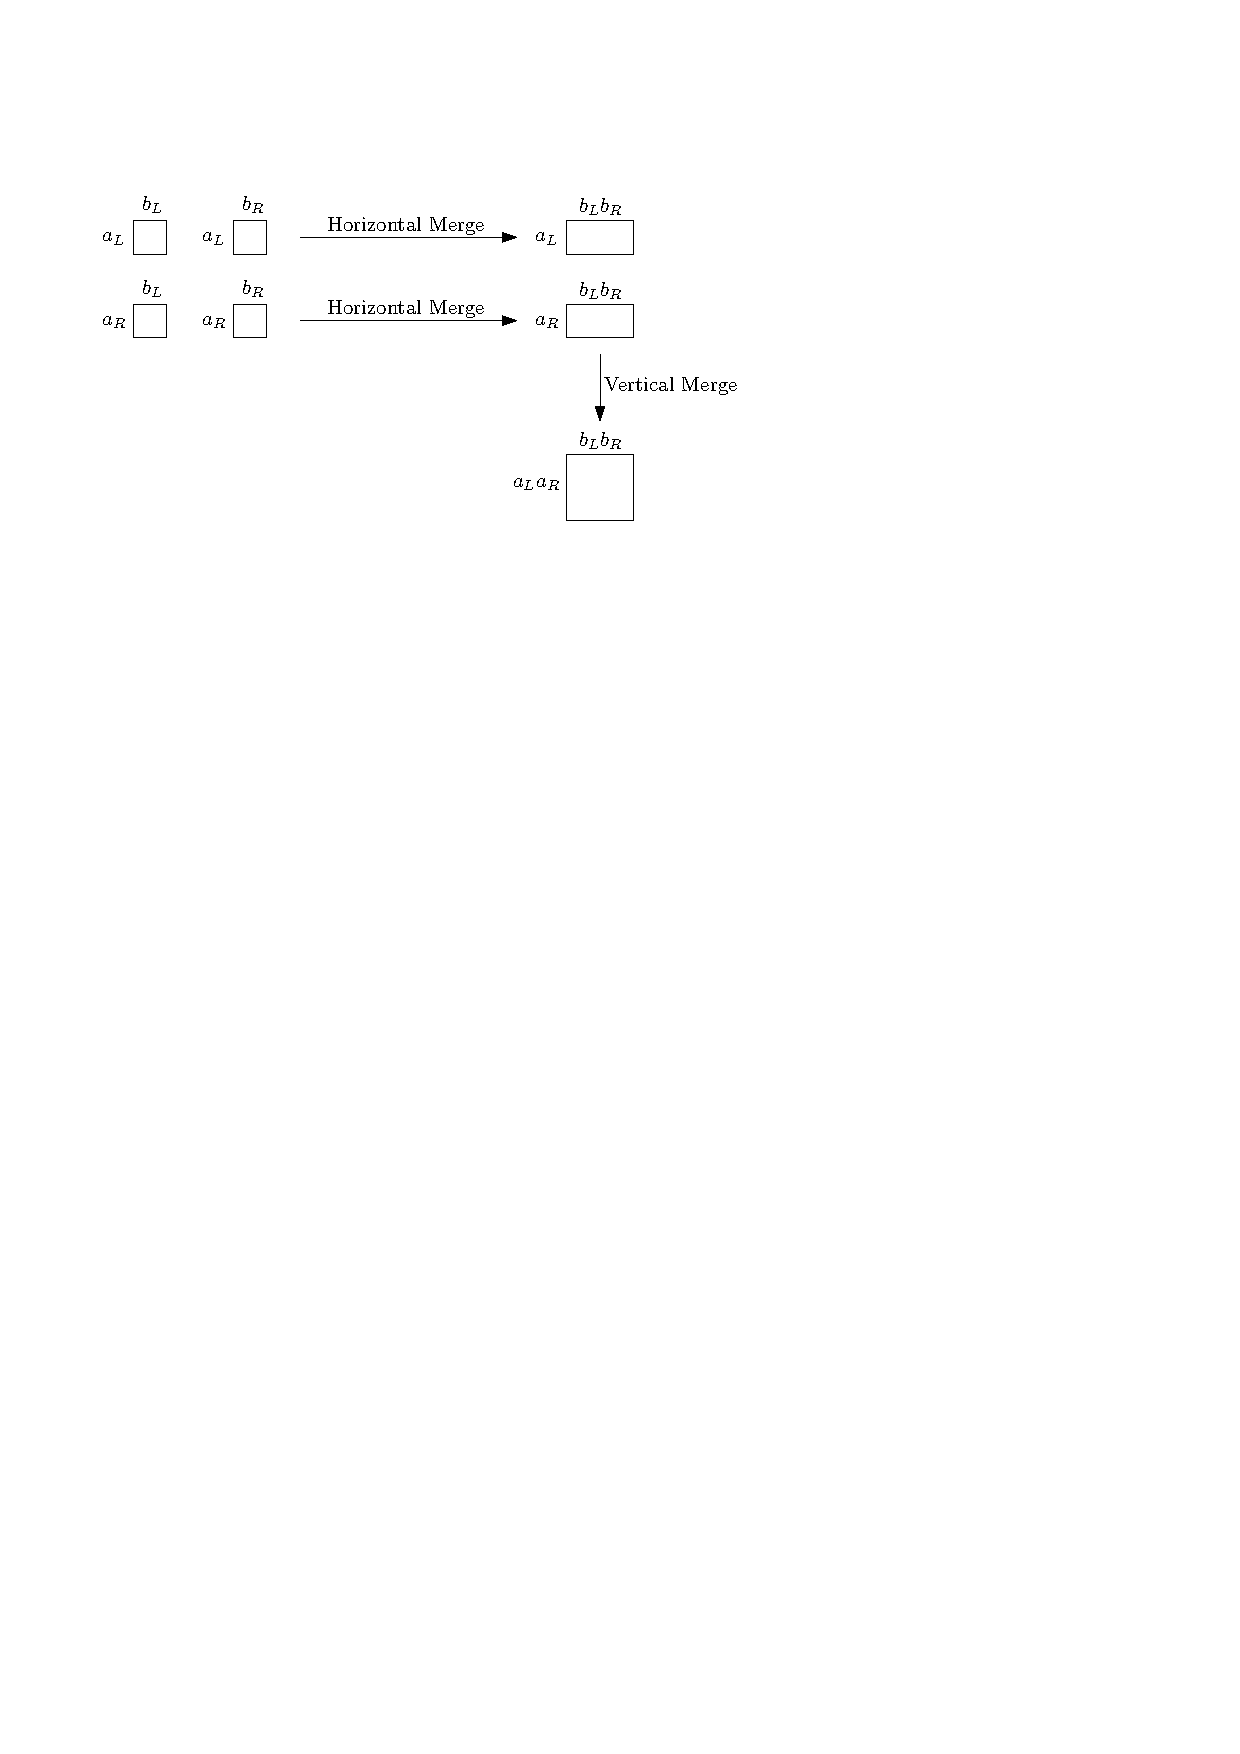
\includegraphics{images/dist_merge}
    \caption{Merging phases of DIST tables from the children to obtain the DIST for the concatenated strings.}
    \label{fig:compression:dist:merge}
  \end{figure}

  \item[Productions associated with substring] For this type of productions a merging approach is also employed. Depending on what side of the path the node was selected, its left/right child is chosen accordantly, and then they are recursively solved and merged together as in the previous case.
\end{description}
Since the number of productions is bounded by $O(n^2)$, the time for constructing the dist repository can be build in time $O(n^2 M(x))$ using memorization, where $M(x)$ denotes the time for merging two DIST tables, which for a rational scoring function and the succinct DIST representation takes time $O(x \log{x})$. In total $O(n^2x\log{x})$ time is spend.

\subsubsection{Filling out the dynamical programming table}
The dynamical programming table is filled from top to bottom, left to right. This is done by keeping two columns of the table in memory (could be reduced to a little more than one column), and then $O(x)$ of a row. This specifies the inputs $I$ to the dist table, and the output can then be computed by
\begin{equation}
  \label{eqn:dist-application}
  O[j] = \min_i \{ I[i] + \DIST[i, j] \},
\end{equation}
since the DIST table stores the shortest path from input $i$ to output $j$. Evaluating the above formula directly for every input takes $O(x^2)$ time, which is too much.

If an explicit representation of the DIST tables is used, then this can be evaluated in time $O(x)$ using the SMAWK algorithm (however, this would increase the time needed for constructing the DIST tables).

\subsubsection{Blow-up method}
In order to improve the theoretical running time of the algorithm, a succinct representation of the DIST tables will be employed. It turns out, that it is much easier to make a succinct encoding of the DIST tables for the related problem Longest Common Subsequence (LCS).

The LCS problem can be seen as the edit distance, but where substitutions are not allowed. The approach taken by \todo{cite} is to use whats known as the blow-up technique, where extra special characters are inserted in the input strings, in order to mimic the edit distance metric. This can be done by transforming every symbol $a \in \Sigma$ in the strings to $a\$$, where $\$ \not\in \Sigma$. \todo{Describe/prove why this works.}

This approach results in the strings becoming a factor of $2$ longer. For a simple $O(n^2)$ implementation of the LCS algorithm, this would result in a factor of $2^2 = 4$ slow down. However, for LCS working on compressed strings, the penalty might not be as severe, since the blown up strings compresses well if the original strings compresses well. This follows from, and also gives an algorithm for performing the blow-up, since every terminal in the SLP can be replaced by a non-terminal producing the original terminal and a new terminal producing the $\$$ symbol. Assuming that the SLP contains $T$  terminals before the blow-up, a total of $T + 1$ new productions are added to the SLP.

\subsubsection{Representation of DIST table}
Given two strings $A$ and $B$, a succinct representation of the LCS DIST tables should be constructed. By definition of the $\DIST$ tables it is known that \todo{Upper and lower triangle not well-defined for $\DIST$! Fix this.}
\[
  \DIST_{A,B}[i, j] = \left\{
    \begin{array}{ll}
      lcs(\substr{A}{m - i}{m}, \substr{B}{0}{j})             & \text{if } i < m, j < n \\
      lcs(A, \substr{B}{i - m}{j})                            & \text{if } i \geq m, j < n \\
      lcs(\substr{A}{m - i}{m - (j - n)}, B)                  & \text{if } i < m, j \geq n \\
      lcs(\substr{A}{0}{m - (j - n)}, \substr{B}{i - m}{n})   & \text{if } i \geq m, j \geq n
    \end{array}
  \right. ,
\]
that is, the $\DIST$ can be summarized as the LCS between all prefix-suffix pairs of the two strings $A$ and $B$. A different way of describing the LCS between these prefix-suffix pairs, is by the following definition.
\begin{mydef}
  \label{def:H-table}
  Let $\str{A}{0}{m}$ and $\str{B}{0}{n}$ be strings, then
  \[
    H_{A,B}(i, j) = lcs(A, \substr{?^mB?^m}{i}{j + m})
  \]
  for $i,j \in \{ 0, \dots, m + n \}$ where $? \not\in \Sigma$ denotes a wildcard character matching all other symbols.
\end{mydef}
The precise correspondence between the $H$-table of \cref{def:H-table} and the $\DIST$ tables, is given by the following lemma.
\begin{lemma}
  \label{lemma:dist-H-relation}
  \[
  DIST[i, j] = H(i, j) + \left\{
    \begin{array}{ll}
      i - m             & \text{if } i < m, j < n \\
      0                 & \text{if } i \geq m, j < n \\
      (i - m) + (n - j) & \text{if } i < m, j \geq n \\
      n - j             & \text{if } i \geq m, j \geq n
    \end{array}
  \right.
  \]
  \begin{proof}
    The lemma follows almost directly by the definition of the DIST, $H$-table and $lcs$ function, by splitting the claim up into the four different cases of the statement.
    \begin{description}
      \item[\circled{1}] For $i \in \{0, \dots, m\}, j \in \{0, \dots, n\}$,
       \begin{align*}
         H(i, j) &= lcs(A, \substr{?^mB?^m}{i}{j + m}) = lcs(A, ?^{m - i}(\substr{B}{0}{j})) \\
                 &= (m - i) + lcs(\substr{A}{m - i}{m}, \substr{B}{0}{j}) = \DIST[i, j] + m - i
       \end{align*}

      \item[\circled{2}] For $i \in \{m, \dots, m + n\}, j \in \{0, \dots, n\}$,
        \[
          H(i, j) = lcs(A, \substr{?^mB?^m}{i}{j + m}) = lcs(A, \substr{B}{i - m}{j}) = \DIST[i, j]
        \]

      \item[\circled{3}] For $i \in \{0, \dots, m\}, j \in \{n, \dots, n + m\}$,
        \begin{align*}
          H(i, j) &= lcs(A, \substr{?^mB?^m}{i}{j + m}) = lcs(A, ?^{m - i}B?^{j - n}) \\
                  &= (m - i) + (j - n) + lcs(\substr{A}{m - i}{m - (j - n)}, B) \\
                  & = (m - i) + (j - n) + \DIST[i, j]
        \end{align*}

      \item[\circled{4}] For $i \in \{m, \dots, m + n\}, j \in \{n, \dots, n + m\}$,
        \begin{align*}
          H(i, j) &= lcs(A, \substr{?^mB?^m}{i}{j + m}) = lcs(A, \substr{B}{i - m}{n}?^{j - n}) \\
                  &= (j - n) + lcs(\substr{A}{0}{m - (j - n)}, \substr{B}{i - m}{n}) = (j - n) + \DIST[i, j]
        \end{align*}
    \end{description}
  \end{proof}
\end{lemma}
An important property of the $H$-table is that it is simple unit-monge \todo{Cite (and prove?)} \todo{Introduce all the matrix terminologies}.
This means, that $H_{A,B}(i, j) = j - (i - m) - P^{\Sigma}(i, j)$ for some permutation matrix $P$ of size $m + n - 1$. Therefore, the permutation matrix $P$, which can be represented in linear space, encodes the $H$-table, and thereby also the $\DIST$-table.

What remains is to ensure that the merge and apply operations operations on the $\DIST$ table can be computed efficiently using only the permutation matrix representation.

\subsubsection{Merging of $\DIST$ tables}
The following definition will come in handy:
\begin{mydef}
  Let $P_{A'}$ and $P_{A''}$ be permutation matrices describing the $\DIST$ tables for the strings $\str{A'}{0}{m'}$ and $\str{A''}{0}{m''}$ respectively. Then, we define
  \[
    IC'_{P_{A'}} = \begin{pmatrix}
      I^{m'' \times m''} & 0 \\
      0 & P_{A'}
    \end{pmatrix}, \quad
    IC''_{P_{A''}} = \begin{pmatrix}
      P_{A''} & 0 \\
      0 & I^{m' \times m'}
    \end{pmatrix}.
  \]
  Notice that both of these new matrices are also permutation matrices, and that they can be efficiently computed by a single scan of the original matrices.

  The following convenient fact that will be useful later, follows directly from the definition of the $\Sigma$-operator:
  \[
    {IC'_{P_{A'}}}^{\varsigma} = \begin{pmatrix}
      (I^{m'' \times m''})^{\varsigma} & 0 \\
      0 & P_{A'}^{\varsigma}
    \end{pmatrix}, \quad
    {IC''_{P_{A''}}}^{\varsigma} = \begin{pmatrix}
      P_{A''}^{\varsigma} & 0 \\
      0 & (I^{m' \times m'})^{\varsigma}
    \end{pmatrix},
  \]
  where $\varsigma$ denotes the $\Sigma$ operator, but where the last row and the first column are removed.
\end{mydef}

\paragraph{Vertical merge}
Now it will be explained how a vertical merge between $A'$ and $A''$ can be found only giving the succinct representation of the DIST tables $\DIST_{A',B}$ and $\DIST_{A'',B}$. From a straight forward analysis of the LCS graph described by the $\DIST$ tables, it is found that:
\begin{claim}
  \label{claim:dist-vertical-merge}
  \item[\circled{1}]: For $i \leq m'', j \leq n + m''$:
    \[
      \DIST_{A'A'',B}[i, j] = \DIST_{A'',B}[i, j]
    \]
  \item[\circled{2}]: For $i \geq m'', j \geq n + m''$:
    \[
      \DIST_{A'A'',B}[i, j] = \DIST_{A',B}[i - m'', j - m''].
    \]
  \item[\circled{3}]: For $i \geq m'', j \leq n + m'$:
    \[
      \DIST[i, j] = \max_{k \in \{0, \dots, n\} } \left\{ \DIST_{A',B}[i - m'', k] + \DIST_{A'',B}[m'' + k, j] \right\}
    \]
  \begin{proof}
    Straight forward from the meaning of the $\DIST$ tables in term of the dynamic programming table by the simple LCS algorithm. \todo{Insert illustrative figure?}
  \end{proof}
\end{claim}
%
For case \circled{3}, the result from \cref{claim:dist-vertical-merge} can be further expanded to find
\begin{align*}
  \DIST_{A'A'',B}[i, j] &= \max_{k \in \{0, \dots, n\} } \left\{ \DIST_{A',B}[i - m'', k] + \DIST_{A'',B}[m'' + k, j] \right\} \\
              &=  \begin{aligned}
                    \max_k \left\{
                      H_{A',B}(i - m'', k) + \left\{
                        \begin{array}{ll}
                          i - m & \text{if } i - m'' < m' \\
                          0     & \text{o/w}
                        \end{array} \right. \right. \\
                      \left. +\,\,H_{A'',B}(m'' + k, j) + \left\{
                        \begin{array}{ll}
                          n - j & \text{if } j \geq n \\
                          0     & \text{o/w}
                        \end{array} \right.
                    \right\}
                 \end{aligned}\\
              &= \max_k \left\{ H_{A',B}(i - m'', k) + H_{A'',B}(m'' + k, j) \right\}
                  + \begin{cases}
                      (i - m) + (n - j)   & \text{if } i < m, j \geq n \\
                      i - m               & \text{if } i < m, j < n \\
                      n - j               & \text{if } i \geq m, j \geq n \\
                      0                   & \text{if } i \geq m, j < n
                    \end{cases}.
\end{align*}
Therefore \cref{lemma:dist-H-relation} now implies that $H_{A'A'',B}(i, j) = \max_k \left\{ H_{A',B}(i - m'', k) + H_{A'',B}(m'' + k, j) \right\}$. This expression can further be written out, to find
\begin{align*}
  H_{A'A'',B}(i, j) &= \max_k \left\{ H_{A',B}(i - m'', k) + H_{A'',B}(m'' + k, j) \right\} \\
                    &= \max_k \left\{ k - (i - m'' - m') - P_{A'}^{\Sigma}(i - m'', k) + j - (k + m'' - m'') - P_{A''}^{\Sigma}(k + m'', j) \right\} \\
                    &= j - (i - m) + \max_k \left\{ -\left( P_{A'}^{\Sigma}(i - m'', k) + P_{A''}^{\Sigma}(k + m'', j) \right)  \right\} \\
                    &= j - (i - m) - \min_k \left\{ P_{A'}^{\Sigma}(i - m'', k) + P_{A''}^{\Sigma}(k + m'', j) \right\}.
\end{align*}
Now \cref{def:H-table} gives that
\begin{align*}
  P_{A'A''}^{\Sigma}(i - m'', j) &= \min_k \left\{ P_{A'}^{\Sigma}(i - m'', k) + P_{A''}^{\Sigma}(k + m'', j) \right\} \\
                                 &= \min_k \{ {IC'_{P_{A'}}}^{\Sigma}(i, k) + {IC''_{P_{A''}}}^{\Sigma}(k, j) \},
\end{align*}
which reduces this case to min-multiplying two simple unit-Monge matrices, which can be solved in time $O(n \log{n})$ by \todo{cite}.

For case \circled{1} where $i \leq m'', j \leq n + m''$, the definition of the $\DIST$ table yields
\begin{align*}
  \DIST_{A'A'',B}[i, j] &= H_{A'A'',B}(i, j) + \left\{
    \begin{array}{ll}
      i - m             & \text{if } j < n \\
      (i - m) + (n - j) & \text{if } j \geq n
    \end{array}
  \right. \\
  &= (i - m) + j - (i - m) - P_{A'A'',B}^\Sigma(i, j) + \left\{
    \begin{array}{ll}
      0             & \text{if } j < n \\
      (n - j)       & \text{if } j \geq n
    \end{array}
  \right. \\
  &= j - P_{A'A'',B}(i, j) + \left\{
    \begin{array}{ll}
      0             & \text{if } j < n \\
      n - j         & \text{if } j \geq n
    \end{array}
  \right.
\end{align*}
By a similar analysis of the statement given by \cref{claim:dist-vertical-merge}, it is found that:
\begin{align*}
  \DIST_{A'A'',B}[i, j] &= \DIST_{A'',B}[i, j] = H_{A'',B}(i, j) + \left\{
    \begin{array}{ll}
      i - m''             & \text{if } j < n \\
      (i - m'') + (n - j) & \text{if } j \geq n
    \end{array}
  \right. \\
  &= \dots = j - P_{A'',B}^{\Sigma}(i, j) + \left\{
    \begin{array}{ll}
      0             & \text{if } j \geq n \\
      n - j         & \text{if } j < n
    \end{array}
  \right.
\end{align*}
Subtracting the two expressions yields $P_{A'',B}^{\Sigma}(i, j) = P_{A'A'',B}^{\Sigma}(i, j)$. It can be noticed that this conforms nicely with the computation carried out in case \circled{1}. Writing from the computation from case \circled{1},
\begin{align*}
  \circled{*} &= \min_{k \in \{0,\dots,n+m\}} \{ {IC'_{P_{A'}}}^{\Sigma}(i, k) + {IC''_{P_{A''}}}^{\Sigma}(k, j) \} \\
  &= \min\left\{
       \min_{k \in \{0,\dots,i\}}{P_{A'',B}^{\Sigma}(k, j)},
       \min_{k \in \{i + 1, n + m\}}\left\{ k - i + \left\{ % A row <= m'' in IC' is like: 0 ... 0 1 2 3 4 ...
        \begin{array}{ll}
          P_{A'',B}^{\Sigma}(k, j) & \text{if } k \leq n + m'' \\
          0                        & \text{if } k > n + m''
        \end{array}
       \right. \right\}
     \right\}.
\end{align*}
%
\begin{claim}
  \label{claim:bounding-sigma}
  The following bound is valid $\forall k \in \mathbb{N}: i + k \leq n + m''$:
  \[
    P_{A''}^{\Sigma}(i, j) \leq k + P_{A''}^{\Sigma}(i + k, j)
  \]
  \begin{proof}
    Follows almost directly from decreasing unit monotonicity of the $\Sigma$-operator used on permutation matrices in both coordinates (only the $i$ coordinate monotonicity used here).
  \end{proof}
\end{claim}
Using \cref{claim:bounding-sigma} at the boundary condition $i + k = n + m''$, it is found that $P_{A''}^{\Sigma}(i, j) \leq n + m'' - i + P_{A''}^{\Sigma}(n + m'', j) = n + m'' - i$. Hence, by first using decreasing unit monotonicity of the $\Sigma$-operator and \cref{claim:bounding-sigma} followed by the claim at the boundary condition, it is found that:
\[
  \circled{*} = \min\{ P_{A''}^{\Sigma}(i, j), \min_{k \in \{n+m'', \dots, n+m\}} \{ k - i \} \}
              = P_{A''}^{\Sigma}(i, j)
\]
Hence, the min-product computed in case \circled{3} also gives the correct result for case \circled{1}.

Case \circled{2} follows by almost the same arguments as case \circled{1}. First \cref{lemma:dist-H-relation} and the definition of the $H$-table is used on \cref{claim:dist-vertical-merge} yielding
\begin{align*}
  \DIST_{A'A'',B}[i, j] &= \DIST_{A',B}[i - m'', j - m''] \\
    &= H_{A',B}(i - m'', j - m'') +
      \begin{cases}
        (i - m'' - m') + (n - (j - m'')) & \text{if } i - m'' < m' \\
        n - (j - m'')                    & \text{if } i - m'' \geq m'
      \end{cases} \\
    &= n + m'' - j + H_{A',B}(i - m'', j - m'') +
      \begin{cases}
        i - m   & \text{if } i < m \\
        0       & \text{o/w}
      \end{cases} \\
    &= n - (i - m) - P_{A',B}^{\Sigma}(i - m'', j - m'') +
      \begin{cases}
        i - m   & \text{if } i < m \\
        0       & \text{o/w}
      \end{cases}
\end{align*}
Similarly writing out directly from the definition, it is found that
\begin{align*}
  \DIST_{A'A'',B}[i, j] &= H_{A'A'',B}(i, j) +
    \begin{cases}
      (i - m) + (n - j) & \text{if } i < m \\
      n - j             & \text{if } i \geq m
    \end{cases} \\
  &= n - (i - m) - P_{A'A'',B}^{\Sigma}(i, j) +
    \begin{cases}
      i - m & \text{if } i < m \\
      0     & \text{if } i \geq m
    \end{cases}
\end{align*}
This implies that $P_{A'A'',B}^{\Sigma}(i, j) = P_{A',B}^{\Sigma}(i - m'', j - m'')$. As will be seen, this is also what is computed by the min-multiplication in case \circled{3}. Writing out the result of the min-multiplication, it is found that
\begin{align*}
  \circled{*} &= \min_{k\in \{ 0, \dots, n + m \}} { {IC'_{P_{A'}}}^{\Sigma}(i, k) + {IC''_{P_{A''}}}^{\Sigma}(k, j) } \\
              &=  \begin{aligned} \min
                    &\left\{
                      \min_{k \in \{0, \dots, m''\}} { P_{A'}^{\Sigma}(k, n + m'') + I^{\Sigma}(0, j - (n + m'')) }, \right. \\
                    &\left.
                      \min_{k \in \{m', \dots, n + m''\}} {P_{A'}^{\Sigma}(i - m'', k - m'') + I^{\Sigma}(0, j - (n + m''))}, \right. \\
                    &\left.
                      \min_{k \in \{ n + m'', \dots, n + m \}} {P_{A'}^{\Sigma}(i - m'', k - m'') + I^{\Sigma}(k - (n + m''), j - (n + m''))}
                    \right\}
                  \end{aligned}
\end{align*}
Notice that the second case always dominates the first, hence the second case can safely be removed from the minimization. Furthermore, the third case can be spitted to obtain
\begin{align*}
  \circled{*} &=  \begin{aligned} \min
                    &\left\{
                      n + m'' + j - n - m'',
                      \min_{k \in \{n + m'', j\}} {j - k + P_{A'}^{\Sigma}(i - m'', k - m'')}, \right.
                    \left.
                      \min_{k \in \{j, \dots, n + m\}} {P_{A'}^{\Sigma}(i - m'', k - m'')}
                    \right\}
                  \end{aligned} \\
              &= \begin{aligned} \min
                    &\left\{
                      j,\quad
                      \min_{k \in \{j, \dots, n + m\}} {j - k + P_{A'}^{\Sigma}(i - m'', k - m'')},\quad
                      P_{A'}^{\Sigma}(i - m'', j - m'')
                    \right\}
                  \end{aligned}
\end{align*}
\begin{claim}
  \label{claim:bounding-sigma-col}
  The following bound is valid $\forall a \in \mathbb{N}: j - a \geq 0$:
  \[
    P_{A'}^{\Sigma}(i - m'', j) \leq a + P_{A'}^{\Sigma}(i - m'', j - a)
  \]
  \begin{proof}
    Follows from unit monotonicity of the $\Sigma$-operator on permutation matrices.
  \end{proof}
\end{claim}
By applying \cref{claim:bounding-sigma-col} with $a = j - k$, it is found that
\[
  P_{A'}^{\Sigma}(i - m'', j - m'') \leq (j - k) + P_{A'}^{\Sigma}(i - m'', j - m'' - (j - k)) = (j - k) + P_{A'}^{\Sigma}(i - m'', k - m'').
\]
This eliminates the middle case of the minimization in $\circled{*}$. Moreover, \cref{claim:bounding-sigma-col} is used to find that
\[
  P_{A'}^{\Sigma}(i - m'', j - m'') \leq (j - m'') + P_{A'}^{\Sigma}(i - m'', 0) = j - m'' \leq j,
\]
which directly gives that $\circled{*} = P_{A'}^{\Sigma}(i - m'', j - m'')$. Therefore the min-multiplication can also be used to solve case \circled{2}. Therefore two $\DIST$ tables can be merged vertically by a single min-multiplication taking $O(x \log{x})$ time.

\paragraph{Horizontal merge}
The horizontal merge will be carried out by means of a vertical merge. In order to do this, it should be efficient to compute $\DIST_{B,A}$ from $\DIST_{A,B}$. It turns out that this indeed easy. In order to see this, first notice that
\begin{claim}
  \label{claim:H_string_switch_relation}
  For all $i, j \in \{0, \dots, n + m\}$ the following identity holds
  \[
    H_{A,B}(i, j) = (m - i) - (n - j) + H_{B,A}(n + m - i, n + m - j)
  \]
  \begin{proof}
    The proof is a case analysis of \cref{def:H-table}.
    \begin{description}
      \item[\circled{1}]: For $i \in \{0, \dots, m\}, j \in \{0, \dots, n\}$
        \begin{align*}
          H_{A,B}(i, j) &= (m - i) + lcs(\substr{A}{m - i}{m}, \substr{B}{0}{j}) \\
            &= (m - i) + lcs(\substr{B}{0}{j}, \substr{A}{m - i}{m}) \\
            &= (m - i) - (n - j) + lcs(B, \substr{m - i}{m} ?^{n - j}) \\
            &= (m - i) - (n - j) + lcs(B, \substr{?^nA^n}{n + m - i}{m + n + n - j}) \\
            &= (m - i) - (n - j) + H_{B,A}(n + m - i, n + m - j)
        \end{align*}

      \item[\circled{2}]: For $i \in \{m, \dots, m+n\}, j \in \{0, \dots, n\}$
        \begin{align*}
          H_{A,B}(i, j) &= lcs(A, \substr{B}{i - m}{j}) = lcs(\substr{B}{i - m}{j}, A) \\
            &= lcs(B, \substr{?^n A ?^n}{n - (i - m)}{n + m + (n - j)}) - (i - m) - (n - j) \\
            &= (m - i) - (n - j) + H_{B,A}(m + n - i, m + n - j)
        \end{align*}

      \item[\circled{3}]: For $i \in \{0, \dots, m\}, j \in \{n, \dots, n+m\}$
        \begin{align*}
          H_{A,B}(i, j) &= (m - i) - (n - j) + lcs(\substr{A}{m - i}{m - (j - n)}, B) \\
            &= (m - i) - (n - j) + lcs(B, \substr{?^n A ?^n}{m + n - i}{m + n - (j - n)}) \\
            &= (m - i) - (n - j) + H_{B,A}(m + n - i, m + n - j)
        \end{align*}

      \item[\circled{4}]: For $i \in \{m, \dots, m+n\}, j \in \{n, \dots, n+m\}$
        \begin{align*}
          H_{A,B}(i, j) &= (j - n+ lcs(\substr{A}{0}{m - (j - n)}, \substr{B}{i - m}{n})) \\
            &= (j - n) + lcs(\substr{B}{i - m}{n}, \substr{A}{0}{m + n - j}) \\
            &= (j - n) + lcs(B, \substr{?^n A ?^n}{n - (i - m)}{n + m + n - j}) - (i - m) \\
            &= (m - i) - (n - j) + H_{B,A}(n + m - i, m + n - j)
        \end{align*}
    \end{description}
  \end{proof}
\end{claim}
%
\begin{claim}
  \label{claim:sum_top_described_as_sum_bottom}
  For all $i, j \in \{0, \dots, n + m\}$ it is the case that
  \[
    \sum_{\hat{i} \in \{i, \dots, n + m\}\atop \hat{j} \in \{ 0, \dots, j \}} P_{B,A}(m + n - \hat{i}, m + n - \hat{j})
      = j - i + P_{B,A}^{\Sigma}(m + n - i, m + n - j)
  \]
  \begin{proof}
    Since $P_{B,A}$ is a permutation matrix, it contains exactly one $1$ in every row/column. Therefore the sum over the top-right area, can be found by taking the sum over the entire matrix and subtract the left and bottom part, and then add the double counted overlap \todo{See figure ...}. This gives that
    \begin{align*}
      &\sum_{\hat{i} \in \{i, \dots, n + m\}\atop \hat{j} \in \{ 0, \dots, j \}} P_{B,A}(m + n - \hat{i}, m + n - \hat{j}) \\
      = &(n + m) - (m + n - j) + ((m + n) - (m + n - i) + P_{B,A}^{\Sigma}(m + n - i, m + n - j)) \\
      = &j - i + P_{B,A}^{\Sigma}(m + n - i, m + n - j).
    \end{align*}
  \end{proof}
\end{claim}

\begin{lemma}
  \label{lemma:swap_strings}
  Assuming $P_{A,B}$ is the permutation matrix encoding $\DIST_{A,B}$, the $\DIST$-table $\DIST_{B,A}$ is encoded by the permutation matrix $P_{B,A}$ where,
  \[
    P_{B,A}(m + n - i, m + n - j) = P_{A,B}(i, j).
  \]
  Notice that the transformed permutation matrix $P_{B,A}$ can easily be computed in linear time by a sweep over its rows.
  \begin{proof}
    It is needed to show that the $H$-table corresponding to the permutation matrix $P_{B,A}$ conforms to \cref{claim:H_string_switch_relation}.
    \begin{align*}
      H_{A,B}(i, j) &= j - (i - m) - P_{A,B}(i, j) \\
        &= j - (i - m) - \sum_{\hat{i} \in \{i,\dots,n+m\}\atop \hat{j} \in \{0, \dots, j\}} P_{A,B}(\hat{i}, \hat{j}) \\
        &= j - (i - m) - \sum_{\hat{i} \in \{i, \dots, n + m\}\atop \hat{j} \in \{ 0, \dots, j \}} P_{B,A}(m + n - \hat{i}, m + n - \hat{j}) \\
        &\overset{\text{\cref{claim:sum_top_described_as_sum_bottom}}}{=} j - (i - m) - (j - i + P_{B,A}^{\Sigma}(m + n - i, m + n - j)) \\
        &= m - P_{B,A}^{\Sigma}(m + n - i, m + n - j) \\
        &= m - \left( (n + m - j) - ((n + m - i) - n) - H_{B,A}(n + m - i, n + m - j) \right) \\
        &= (m - i) - (n - j) + H_{B,A}(n + m - i, n + m - j)
    \end{align*}
    This matches the statement of \cref{claim:H_string_switch_relation}, which completes the proof.
  \end{proof}
\end{lemma}
%
Follow \cref{lemma:swap_strings} a horizontal merge can be carried out by first swapping the strings, then performing a vertical merge, and then swapping the strings of the merged $\DIST$ table again. Since swapping the strings runs in time $O(x)$, the total time of a horizontal merge is bounded by the time of the vertical merging. Hence, the total time of either of the merge routines is bounded by $O(x\log{x})$.

\subsubsection{Application of $\DIST$ tables}
When filling out a block in the grid with input $I$, the output is given by
\begin{align*}
  O[j] &= \max_i \left\{ I[i] + \DIST[i, j] \right\} \\
    &= \max_i \left\{ I[i] + H(i, j) + \left\{
      \begin{array}{ll}
        i - m             & \text{if } i < m, j < n \\
        0                 & \text{if } i \geq m, j < n \\
        (i - m) + (n - j) & \text{if } i < m, j \geq n \\
        n - j             & \text{if } i \geq m, j \geq n
      \end{array}
    \right. \right\} \\
    &= \max_i\left\{ \left( I[i] + \left\{
      \begin{array}{ll}
        i - m     & \text{if } i < m \\
        0         & \text{o/w.}
      \end{array}
    \right. \right) + H(i, j) \right\} + \left\{
      \begin{array}{ll}
        n - j     & \text{if } j \geq n \\
        0         & \text{o/w.}
      \end{array}
    \right. .
\end{align*}
Hence, the output can be evaluated by max-multiplying the $H$ table with a slight perturbation of the input array, followed by an addition for every resulting output. \todo{cite} gave a linear time algorithm for max-multiplying an arbitrary vector with a simple unit-Monge matrix \todo{Describe algorithm?}. This gives a linear time algorithm for applying the $\DIST$ table.


%%%%%%%%%%%%%%%%%%%%%%%%%%%%%%%%%%%%%%%%%%%%%%%%%%%%%%%%%%%%%%%%%%%%%%%

\addcontentsline{toc}{chapter}{Bibliography}
\bibliographystyleA{plain} 
\bibliographyA{refs}
%\addcontentsline{toc}{chapter}{Secondary Bibliography}
%\bibliographystyleB{plain} 
%\bibliographyB{refs} % remove this if you don't need secondary literature

\end{document}

